\chapter{Úvod}
\label{kap:uvod}

Muselo to být někdy v~roce 2010, kdy mi moje kamarádka Alenka do ruky podala
cédéčko s~popiskem ,,Karel Makoň`` se slovy, že si to mám poslechnout. Doma jsem
disk vložil do mechaniky a nechal se unášet slovy, která se mi vryla do paměti:

{\em ,,I v~tomto systému lásky, ať konkrétně vypadá jakkoliv, platí, že tam není
vším to, co dělám, nýbrž důležitou složkou je také to, co nedělám. Víš,
podobnost je v~klepání. Klepání je podobno dělat nedělat, systému dělat,
nedělat. Systému samočinného počítače, jedna, nula, nula, jedna, jedna, nula. Já
žiju ve dvojnosti. Všechno v~ní pulzuje. A taky tento systém, který ze dvojnosti
vede, to je pulzace na vyšší úrovni.``}

Obsah, jakož i podmanivý hlas mluvčího, mne natolik strhly, že jsem se začal
pídit po tom, zda existují od tohoto Karla Makoně další nahrávky. Dozvěděl jsem
se, že ano. Alenka mě odkázala na nějakého doktora Elgra ze Zlína, který jich má
prý mnoho.

Vydal jsem se tedy do Zlína za panem doktorem Elgrem. Usměvavý šedivý pán
s~vyzařováním šlechtice se mi představil jako Vít a uvedl mě do svojí pracovny, jejíž celá stěna byla
pokryta skříněmi zaplněnými kazetami a kotouči. Vyprávěl mi, jak jezdil
s~,,Karlíčkem`` a nahrával každé jeho slovo po desítky let.

Nejdřív se mne zmocnil úžas, pak euforie a nakonec mne polil studený pot při
pomyšlení, že magnetický signál neúprosně slábne a že tento poklad je odsouzen
k~zániku... pokud jej někdo nezdigitalizuje.

Domluvil jsem se s~Vítem, že si budu jeho sbírku po částech půjčovat a celou ji
zdigitalizuji, aby se její obsah uchoval pro další generace. Následující dva
roky jsem strávil přehazováním kazet v~přehrávači a pravidelnými návštěvami
Zlína s~krosnou.

Výsledkem byla sbírka asi tisíce zvukových souborů, které jsem všem přátelům,
kteří o Makoňově díle věděli, rozdal na pevných discích a vystavil ke stažení na
internetu.

Hlavní a urgentní cíl, aby byly nahrávky zachráněny před degradací, se tím
splnil. To byl však začátek věcí.

\section{Motivace k~disertaci}

Hlavním a společným bodem negativní zpětné vazby ke zdigitalizovanému materiálu
bylo, že je v~podstatě nemožné se v~něm vyznat. Ani lidé, kteří byli nahrávání
osobně přítomni, nedokázali najít nějakou pasáž, kterou by si rádi poslechli. Je
sice pravda, že neméně nepřehledná byla sbírka před digitalizací, ale tím, že
byla najednou celá k~dispozici, tento problém vyvstal a nabral na aktuálnosti.

Pojal jsem tedy záměr archiv nejen zachránit a zpřístupnit, ale umožnit jeho
maximální užitek co nejširšímu okruhu zájemců, ať už v~přítomnosti nebo
v~budoucnosti.
Za nejpřínosnější počin se mi jevilo pořízení kompletního
přepisu. Tím by se umožnilo jak vyhledávání, tak jakékoliv další zpracování a
prozkoumávání materiálu.

Přepsat ručně tisíc hodin bylo zcela mimo moje možnosti, byť bych se pokusil
s~pomocí komunity kolem Makoňova odkazu financovat placené přepisovatele nebo
přepisovat svépomocí. Vědomí, že se jedná o mluvené slovo jednoho mluvčího
v~jedné tematické doméně mi skýtala naději na přepis automatický. Navíc vědomí o
existenci lidí, kteří se o nahrávky zajímají právě tak jako já, mne přivedlo
k~nápadu ruční přepis s~automatickým skloubit.
Stál jsem před úkolem designu mluveného korpusu, což přede mnou dělal
např. Crowdy (1993)\cite{crowdy1993spoken}.

Konzultace s~doktorem Ninem Peterkem mi pomohla vytýčit cestu:
\begin{enumerate}
\item{Ručně pořídím přepis několika minut Makoňových nahrávek.}
\item{Vytvořím systém rozpoznávání řeči.}
\item{Natrénuji ho na pořízeném přepisu.}
\item{Pořídím automatický přepis celého korpusu.}
\item{Naprogramuji webovou aplikaci, která umožní uživateli nahrávky přehrávat,
synchronně u toho zobrazovat přepis a opravovat v~něm chyby.}
\item{Opravy od uživatelů budu hromadit a používat jako další trénovací data pro
rozpoznávač.}
\item{Tak se iterativně dopracuji ke kvalitnímu kompletnímu přepisu za pomoci
vlastního úsilí a přispění komunity.}
\end{enumerate}

Architekturu ilustruje obrázek~\ref{fig:arch}

\begin{figure}[htpb]
\includegraphics[scale=1.0]{rc/arch.eps}
\caption{schéma architektury systému}
\label{fig:arch}
\end{figure}

\section{Obsah}

Tato disertační práce má tedy zastřešující cíl uchování, zpřístupnění a
zužitkování mluveného odkazu Ing. Karla Makoně. V rámci tohoto cíle se zabývá
následujícími body:

\begin{itemize}
\item{rozboru samotných dat v~kapitole \ref{kap:data},}
\item{tvorbě systému pro automatický přepis v~kapitole \ref{kap:asr},}
\item{webové aplikaci pro sběr oprav přepisu v~kapitole \ref{kap:webove-rozhrani},}
\item{vyhledávání v~korpusu v~kapitole \ref{kap:vyhledavani}}
\item{a aplikaci vyvinuté technologie na jiná data v kapitole \ref{kap:jina-data}.}
\end{itemize}

Práci uzavírá kapitola \ref{kap:zaver}.
